\documentclass{vldb}

\usepackage{amsmath,amssymb}
\usepackage{stmaryrd}
\usepackage{graphicx}
\usepackage{color}
\usepackage{hyperref}

\newcommand{\comment}[1]{}
\newcommand{\tinysection}[1]{\noindent{\bf #1.}}
\newcommand{\tuple}[1]{{\langle#1\rangle}}
\newcommand{\todo}[1]{\textcolor{red}{#1}}
\newcommand{\note}[1]{\textcolor{blue}{#1}}

\newcommand{\compiler}{DBToaster}
\newcommand{\spe}{Jasper}
\newcommand{\driver}{JDBC}

\newcommand{\targetlang}{Java}
\newcommand{\dsl}{QueryDSL}
\newcommand{\dslurl}{\url{http://www.querydsl.com}}

%\newcommand{\targetlang}{Scala}
%\newcommand{\dsl}{ScalaQuery}
%\newcommand{\dslurl}{\url{http://http://scalaquery.org}}


\toappear{}


\begin{document}
\title{Algorithmic Trading on Order Books with Embedded Queries and Synthesized
Stream Engines}
\numberofauthors{3}
\author{
\alignauthor
Oliver Kennedy\\
\affaddr{EPFL}\\
\email{oliver.kennedy@epfl.ch}
\alignauthor
Yanif Ahmad\\
\affaddr{Johns Hopkins University}\\
\email{yanif@jhu.edu}
\alignauthor
Christoph Koch\\
\affaddr{EPFL}\\
\email{christoph.koch@epfl.ch}}
\maketitle

\begin{abstract}
Algorithmic trading is an exiting area where computer science
meets economics and finance. Algorithmic
trading has gained substantial traction in recent years and is now
responsible
for a majority of the volume traded on key financial exchanges such as
NASDAQ and the London Stock Exchange.
It is an innovation engine for IT since it creates substantial
networking, data management, and computation challenges and
the players in this space have large budgets for IT infrastructure.
High-frequency algorithmic trading companies have
become a key market for high-speed switches, fast computing hardware, and data
management software -- particularly stream processors.

In this demo, we showcase a new platform for algorithmic trading.
It is based on a newly developed stream processing engine
as well as a finanical exchange simulator, a subsystem for replaying
historical data streams of buy and sell orders,
and implementations of various trading strategies.
We also demonstrate out trading strategy design and development environment.
It allows to express the data analysis portions of strategies
declaratively, using SQL on top of representations of the current
market microstructure, such as order books.
It compiles these declarative specifications down into highly efficient
code using our DBToaster compiler for {\em agile views} \cite{KAK2011},
aggressively incremental view maintenance programs that are able to
keep complex materialized SQL aggregate views continuously fresh through
updates to the base data at very high rates.
\end{abstract}

\section{Introduction}



In recent years, algorithmic trading systems have come to account for a majority
of volume traded at the major US and European financial markets (for instance,
for 73\% of all US equity trading volume in the first quarter of 2009
\cite{Iati2009}). The success of automated trading systems depends critically on
strategy processing speeds: trading systems that react faster to market events
tend to make money at the cost of slower systems. Unsurprisingly, algorithmic
trading has become a substantial source of business for the IT industry; for
instance, it is the leading vertical among the customer bases for high-speed
switch manufacturers (e.g., Arista \cite{Becht2010}) and data stream processing.




A typical algorithmic trading system is run by mathematicians who develop
trading strategies and by programmers and systems experts who implement these
strategies to perform fast enough, using mainly low-level programming languages
such as C. Developing trading strategies requires a feedback loop of simulation,
back-testing with historical data, and strategy refinement based on the insights
gained. This loop, and the considerable amount of low-level programming that it
causes, is the root of a very costly {\em productivity bottleneck}\/: in fact,
the number of programmers often exceeds the number of strategy designers by
an order of magnitude.


Trading algorithms often perform a considerable amount of data crunching
and statistical processing that could in principle be implemented using SQL
views, coupled with some relatively straightforward control and trading logic.
%
Differently from other areas of finance such as technical analysis,
where stream processing engines
\cite{abadi-vldbj:03,motwani-cidr:03} can be applied,
data processing in trading algorithms using views cannot be performed by DBMS or
data stream processing systems today: the former are not able to (1) {\em update
their views at the required rates}\/ (for popular stocks, hundreds of orders per
second may be executed, even outside burst times) and the latter are not able to
(2) {\em maintain large enough data state}\/ and support suitable query
languages (non-windowed SQL aggregates) on this state.

%
A data management system that could handle these two requirements would yield a
very substantial productivity increase that can be directly monetized -- the
holy grail of algorithmic trading.

Trading algorithms often perform a considerable amount of data crunching that
could in principle be implemented as SQL views, but cannot be achieved by DBMS
or data stream processing systems today: DBMS are not able to (1) {\em update
their views at the required rates}\/ (for popular stocks, hundreds of orders per
second may be executed, even outside burst times) and stream engines are not
able to (2) {\em maintain large enough data state}\/ and support suitable query
languages (non-windowed SQL aggregates) on this state.
A data management system fulfilling these two requirements would yield a very
substantial productivity increase that can be directly monetized -- the holy
grail of algorithmic trading.



To understand the need to maintain and query a large data state, note that
many stock exchanges provide a detailed view of the market microstructure
through complete bid and ask {\em limit order books}. The bid order book is a
table of purchase offers with their prices and volumes, and correspondingly the
ask order book indicates investors' selling orders. Exchanges execute trades by
matching bids and asks by price and favoring earlier timestamps. Investors
continually add, modify or withdraw limit orders, thus one may view order books
as relational tables subject to high update volumes. The availability of order
book data has provided substantial opportunities for automatic algorithmic
trading.





To illustrate this, we describe the Static Order Book Imbalance (SOBI) trading
strategy. SOBI computes a volume-weighted average price (VWAP) over those orders
whose volume makes up a fixed upper $k$-fraction of the total stock volume in
both bid and ask order books. SOBI then compares the two VWAPs and, based on
this, predicts a future price drift (for example a bid VWAP larger than an ask
VWAP indicates demand exceeds supply, and prices may rise). For simplicity, we
present the VWAP for the bids only:



\begin{verbatim}
select avg(b2.price * b2.volume) as bid_vwap
from   bids b2
where  k * (select sum(volume) from bids)
         > (select sum(volume) from bids b1
            where b1.price > b2.price);
\end{verbatim}
\comment{
Focusing on the $k$-fraction of the order book closest to the current price
makes the SOBI strategy less prone to attacks known as {\em axes}\/ (large
tactical orders far from the current price that will thus not be executed but
may confuse competing algorithms).
}


Coming back to our two desiderata, for trading algorithms to be successful, (1)
views such as VWAP need to be maintained and monitored by the algorithms at or
close to the trading rate. However, (2) the views cannot be expressed through
time-, row- or punctuation-based window semantics.






\section{The DBToaster Platform}

We present an example of designing a transition function between database
states, in this case focusing on dynamic data driving view maintenance of
standing queries comprising the visible schema. The underlying conceptual model
of a database management system as a state machine has driven our prior work on
this topic in the DBToaster project [REFS], and here we discuss how the concept
of transitioning entire database states has led to a novel view maintenance
algorithm. Furthermore the need to apply this transition with high frequency
motivates precomputing and compiling the transition function into extremely
efficient code.

This section is intended to convey that our database-as-state model can lead to
significant rethinking of existing methods throughout a data management system,
and novelty, algorithmically and architecturally, in designing a system to
handle dynamic data. Throughout this section, we use the term transition to
refer to both the update itself, and the work required to evolve the database
following the application of the update to base tables.

\vspace{1mm}
\subsection{View Maintenance in DBToaster}
Given a database state, existing view maintenance techniques will incrementally
handle transitions to another state for a given update. We can informally
represent this with a triple $\tuple{q,m,q'}$, corresponding to the view query,
the materialization of that query, and the delta query responsible for
maintaining the materialization.
\note{Should talk more about delta queries if you're going to make this the
first mention of it, i.e. with an example}
On an update, view maintenance performs the work: $m_{new} = m_{old} + q'(u)$,
and this is guaranteed to ensure $m_{new} = q(db_{new})$. That is, a
materialized view can be updated with the result of a delta query taking an
update $u$ as an argument, and the view maintenance technique must ensure the
updated view is equivalent to the query result on the modified database. Here,
the delta query can be thought of as a parameterized SQL query, with parameters
corresponding to attributes in the update.

With our conceptual model, we are able to make the
following key insight when taking a holistic approach with the state machine
model, namely that repeatedly applying the same transition with current
techniques results in significantly redundant work. While a transition results
in incremental processing in terms of the part of the database affected by the
update, it is not incremental with respect to the remainder of the database. The
transition evalutes delta queries from scratch on the remainder of the database,
rather than leveraging the fact that this remnant has not changed, and any work
done previously on that portion of the database can be reused.
\note{Diagram here:
\comment{states containing base relations and a query,
transitions for all base relations, each leading to another state. For one of these
neighboring states, we'll repeatedly apply the same transition, highlighting
that the remainder of the base tables do not change, yet the delta queries are
still evaluated from scratch.}
}

To facilitate reuse, we materialize the delta query over the remainder tables,
making it part of the auxiliary state of the database. We refer to this as the
view state, and it is used in our view maintenance approach. Subsequently our
transitions must maintain the view state, leading to the concept of higher-order
delta queries. Higher-order deltas are determined through a recursive processing
of materializing a delta query, and then incrementally maintaining the
materialized result (which would involve further materialization, and delta
queries and so on). That is we can define further triples,
$\tuple{q', m', q''}$, corresponding to the delta query, its materilization,
and a second-order delta query, and so on with $\tuple{q'',m'',q'''}$.
\note{Diagram here.}

This process does not continue forever and terminates given one important
property of computing delta queries: \textit{a delta query is often simpler than
its parent query}. In particular \textit{k}-th order delta query, $q^k$ has
fewer input relations than a \textit{k-1} order query $q^{k-1}$, but additional
parameters corresponding to attributes that are present in $q^{k-1}$. This
provides an informal overview of our view maintenance approach, and we present
an algorithm below to compute both the view state being materialized and the
higher-order delta queries that maintains the view state. The algorithm yields a
\textit{transition program}, essentially trigger function that efficiently
executes a transition from one database to another, including both the visible
and auxiliary state. For the view maintenance problem, the transition program is
simply a sequences of updates to materialized views by delta queries, each
update being of a different order.

\vspace{1mm}
\subsection{Compiling Queries to Transition Programs}
\noindent To present our algorithm, we first describe our query representation,
tailored for incremental processing, and a simple and powerful set of transformations
that we use to simplify and optimize queries.

\tinysection{Query Language}
\noindent Our query language is described by the following EBNF:

\def \calcsum{\mbox{Sum}}
\def\calceq{\mbox{{\tt =}}}
\def\calcgt{\mbox{{\tt >}}}
\def\calcgte{\mbox{{\tt >=}}}
\def\calclte{\mbox{{\tt <=}}}
\def\calclt{\mbox{{\tt <}}}

\def \q{q}
\def \qa{q_1}
\def \qb{q_2}
\def \v#1{\mbox{#1}}
\def \vv#1{\mbox{{\tiny #1}}}
\def \z{\mathbb{Z}}

\vspace{-3mm}
\begin{align*} 
\q \; \mbox{::-} &
  \;    c \;|\; x
  \;|\; R(\vec{x}) \;|\; m(\vec{x},\vec{y})
\\
| & \; \calcsum(\vec{x}, \q)
  \;|\; \q + \q \;|\; \q * \q  \;|\; -\q
  \;|\; \q \; \theta \; 0 \;|\; x := \q
\end{align*}

The grammar represents basic terms of queries such as constants, variables, and
relations $R$ (with attributes $\vec{x}$). We represent materialized views, $m$,
and refer to them as \textit{maps} since these are the underlying in-memory data
structures. Materialized views, or maps, are parameterized SQL queries that
accept parameters $\vec{x}$, and yield schema $\vec{y}$.
Specifically, a map is a \textit{materialized} parameterized query,
where we materialize for all parameter values seen during continuous query
execution (the \textit{active domain} of the parameter).
The intuition behind the representation of views as parameterized SQL comes from
our need to materialize delta queries, which have parameters according to the
update they handle.

For complex terms, the grammar captures sum aggregates
$Sum(\vec{x},q)$ with group-by attributes $\vec{x}$, three generalized
arithmetic operators, addition, multiplication and additive inverse, a
comparison operator ($\theta \in \{=,\neq,<,\leq,>,\geq\}$), and variable
assignment ($:=$). For readability, we write $\calcsum(\q)$ if an aggregate
has no group-bys, and simplify the syntax of comparison as $\theta(\q)$ since
the RHS is 0. 
Our language is quite rich, for example it can represent nested scalar
queries such as the VWAP query in Section [REF]:

\comment{
\begin{verbatim}
select sum(price * vol) from bids b0
where 0.25 * (select sum(b1.vol) from bids b1) >
     (select sum(b2.vol) from bids b2
      where b2.price > b0.price)
\end{verbatim}
}

\vspace{-3mm}
\begin{align*}
\calcsum(
& B(\v{P0,V0}) * \v{P0} * \v{V0} *\\
& \calcgt(0.25 * \calcsum(B(\v{P1,V1}) * \v{V1}) \\
& \qquad \; \; - \calcsum(B(\v{P2,V2}) * \v{V2} * \calcgt(\v{P2-P0}))))
\end{align*}

We briefly discuss expression semantics, starting with maps. Strictly speaking,
\textit{all of the expressions in our grammar (i.e. queries) represent maps},
and maps associate keys to values. Recall our analogy between maps
$m(\vec{x},\vec{y})$ and parameterized SQL queries. Map $m$ has a key
$\tuple{\vec{x},\vec{y}}$, namely the parameters (bound variables, which must be
provided when evaluating a parameterized query) and schema attributes (free
variables, returned by the query). For readability, we use a doubly-indexed map
notation, $m[\vec{x}][\vec{y}]$, instead of writing in pair notation throughout
$m[\tuple{\vec{x}, \vec{y}}]$. We define map values with a generalized multiset
relation [PODS REF] model of a database, where a relation $R$ is a map whose
value yields the cardinality of that tuple in a multiset.

We assume that the user queries provided as input to compilation contain no
maps, only relations and other terms as is standard in SQL. Our compilation
algorithm rewrites queries to include maps. Due to space constraints, we focus
on two arithmetic operations, addition and multiplication. First, we present an
example of addition:

\vspace{-7mm}
\begin{figure}[h]
\begin{minipage}{1in}
\[
\begin{array}{ll|ll|l}
\multicolumn{5}{c}{m1}\\
 a & c & b & d & \\
\hline
 1 & 1 & 2 & 1 & 3 \\
\comment{
 1 & 2 & 4 & 2 & 1 \\
 1 & 2 & 3 & 3 & 4 \\
}
 1 & 2 &   & 4 & 2
\end{array}
\]
\end{minipage}
+
\begin{minipage}{0.85in}
\[
\begin{array}{ll|l|l}
\multicolumn{4}{c}{m2}\\
 a & c & d & \\
\hline
 1 & 1 & 1 & 1 \\
 1 & 2 & 4 & 2 \\
\end{array}
\]
\end{minipage}
=
\begin{minipage}{1in}
\[
\begin{array}{ll|ll|l}
\multicolumn{5}{c}{m1 + m2}\\
 a & c & b & d & \\
\hline
 1 & 1 & 2 & 1 & 3 \\
 1 & 1 &   & 1 & 1 \\
\comment{
 1 & 2 & 4 & 2 & 1 \\
 1 & 2 & 3 & 3 & 4 \\
}
 1 & 2 &   & 4 & 4
\end{array}
\]
\end{minipage}
\end{figure}

\vspace{-3mm}
\noindent Above, we have two maps $m1, m2$, where blanks in columns represent
\textit{holes}. Holes are not the same as nulls, they determine when attributes
can be ignored for consistency across tuples.
\note{Explain consistency.}
Addition is a schemaless union where the result contains the union of
operand maps' parameters and result schemas, and adds the values of map entries.

Next, we discuss multiplication. Multiplication is the key
connective in our language since it performs binding propagation, similarly to
datalog, where one map's result schema contains attributes used for
another map's parameters, as seen in $m1[a][b1,b2] * m2[b2,c][d]$.
Here, $b2$ is propagated from map $m1$ to $m2$. The result of this
operation ensures consistency of $b2$ between maps $m1, m2$ (inconsistent
tuples are not included in the output), for example:

\vspace{-4mm}
\begin{figure}[h]
\begin{minipage}{1in}
\[
\begin{array}{l|ll|l}
\multicolumn{4}{c}{m1}\\
 a & b_1 & b_2 & \\
\hline
 1 & 2 & 4 & 3 \\
 2 & 4 & 1 & 1 \\
 2 & 3 & 2 & 4
\end{array}
\]
\end{minipage}
*
\begin{minipage}{0.85in}
\[
\begin{array}{ll|l|l}
\multicolumn{4}{c}{m2}\\
 b_2 & c & d & \\
\hline
 1 & 1 & 1 & 1 \\
 2 & 2 & 4 & 2 \\
\end{array}
\]
\end{minipage}
=
\begin{minipage}{1in}
\[
\begin{array}{ll|ll|l}
\multicolumn{5}{c}{m1 * m2}\\
 a & c & b_1 & d & \\
\hline
 2 & 1 & 4 & 1 & 1 \\
 2 & 2 & 3 & 4 & 8 \\
\end{array}
\]
\end{minipage}
\end{figure}

\vspace{-3mm}
\noindent Above, $b2$ is excluded from the result key since it is a propagated
attribute. The tuple $\tuple{a=1,b1=2,b2=4 \mapsto 3}$ in $m1$ does not
contribute to the result since there is no consistent value of $b2$ in $m2$.
Multiplication is a generalized equi-join, and in the absence of any
propagation, a generalized Cartesian product that operates on both levels of
maps.
\todo{Explain variables, i.e. we don't materialize attributes but these are
bound from the left.}
Binding propagation is critical for a few reasons: i) for
multiplication with variables, it allows a map's values to be combined with the
variable's value; ii) for multiplication with constraints, it yields maps
with 0-1 values indicating whether entries pass the constraint; iii) for
multiplication with other maps, where it facilitiates equi-joins and correlated
attributes in nested queries.


\comment{
We write these semantics as
$R := \tuple{} \mapsto \vec{x} \mapsto R(\vec{x})$, indicating the map has a key
with no parameters, schema $\vec{x}$, and value given by the cardinality $R(x)$
of the multiset $R$. The \textit{type} of the map is
$R : \tuple{} \mapsto \vec{x} \mapsto \z$, thus the semantics indicates the
result key, and the map value.

The semantics of constants and variables are: $c := \tuple{} \mapsto
\tuple{} \mapsto c$ and $Var(x) := \vec{b} \mapsto \tuple{} \mapsto \vec{b}(x)$.
The latter states that variables get their value from query parameters.
Due to space constraints, we briefly present the semantics of complex terms.


\vspace{-4mm}
\begin{align*}
\calcsum(\vec{y}, \q[\vec{x}][\vec{y}\vec{z}]) := & \;
\vec{x} \mapsto \vec{y} \mapsto \sum_{\vec{z}} \q
\\
\qa[\vec{u}][\vec{v}] + \qb[\vec{w}][\vec{x}] := & \;
\vec{y} \mapsto \vec{z} \mapsto
\qa[\vec{y}][\vec{z}] + \qb[\vec{y}][\vec{z}]
\\
& \mbox{ where $\vec{y} = \vec{u} \cup \vec{w}, \vec{z} = \vec{v} \cup \vec{x}$}
\\
-\q[\vec{x}][\vec{y}] := & \; \vec{x} \mapsto \vec{y} \mapsto -(\q)
\\
\q[\vec{x}][] \; \theta \; 0 := & \; \vec{x} \mapsto \tuple{} \mapsto
                    \begin{cases}
                    1 \ldots \q \; \theta \; 0\\
                    0 \ldots \mbox{otherwise.}
                    \end{cases}
\\
(x := \q[\vec{b}][]) := & \; \vec{b} \mapsto \tuple{x=q} \mapsto 1
\end{align*}

Above, we write typing constraints of subexpressions on the left-hand
side of semantics definitions. Thus a sum aggregate with group-by $\vec{y}$
over a map $q[\vec{x}][\vec{yz}]$ adds up values of $\vec{z}$. 
\note{Talk about consistency.}
The addition operator ($+$) is a schemaless union over both parameters and
result schema of its inputs. Additive inverse simply negates the map value,
preserving its type. Predicates yield maps with 0-1 values, and are constrained
to have no output schema. They are singletons, just like constants and
variables, and in this way, our language supports nested scalar queries such as
nested sum aggregates. Finally variable assignment $x := q$ yields a singleton
map with schema $x$, and key (of value) $q$. This leaves the multiplication
operator, which in our langauge is capable of propagating parameters, much like
datalog. Suppose we have: $\qa[\vec{u}][\vec{v}] * \qb[\vec{w}][\vec{x}] :=$

\vspace{-4mm}
\begin{align*}
& \vec{y} \mapsto
\sum_{\{y\} = \{u\} \Join \{w\}} 
\vec{z} \mapsto
  \sum_{\{z\} = \{v\} \Join \{x\}}
  \qa[\vec{y}][\vec{z}] * \qb[\vec{y}][\vec{z}]
\\
& \ldots \mbox{when $\vec{v} \cap \vec{w} = \emptyset$}
\\
& \vec{y} \mapsto
\sum_{\{y\} = \{u\} \Join \{b\}} 
\vec{z} \mapsto
  \sum_{\{z\} = \{v\} \Join \{ax\}}
  \qa[\vec{y}][\vec{z}] * \qb[\vec{y}][\vec{z}]
\\
& \ldots \mbox{otherwise, where $\vec{v} \cap \vec{w} = \vec{a}, 
\vec{w} - \vec{v} = \vec{b}$}
\end{align*}

Above, the first case describes when no propagation occurs. The result map has
parameters and schema according to the join of the operands' keys and value as a
product of operand values. In the second case we have propagation of the LHS
query's result schema being bound as parameters in the RHS query. Thus the
result map does not consider propagated attributes as parameters itself.
}


\vspace{0.5mm}
\tinysection{Query Transformations}
We present a set of query transformations, through examples for brevity, that
can be used by our algorithm to simplify and optimize queries.
\comment{
The first is a canonicalization of queries into a \textit{recursively
polynomial} form. A polynomial query is a query represented as a sum of
\textit{monomials}, where monomials are products of any other type of query
(constraints, aggregates, etc. but not sums or products). This is a polynomial
with two monomials:
\begin{align*}
\calcsum( & R(\v{A,B}) * S(\v{C,D}) * \calcgt(\v{B}-\v{C}) *
\calceq(\v{A}-\v{D})) * \\
& \calcsum(T(\v{E,F}) * \v{E}) + -\calcsum(U(\v{G,H}) * \calceq(\v{H}-5))
\end{align*}
The following query is not a polynomial:

$\calcsum(R(\v{A,B}) + (S(\v{C,D}) * \v{C})) *
 \calcsum(T(\v{E,F}) * \calceq(\v{E}-10))$

\noindent because of the addition inside the first sum aggregate. Due to nested
queries, we define our normal form recursively, where each nested
query is also in polynomial form. We require this normal form to easily apply
the following simplifications.
}

To simplify queries, we apply unification, which facilitates variable
elimination, and then factorization, which separates a complex monomial into a
product of simpler monomials. First we give an example of unification and
variable elimination: \todo{xxx}

Now, we demonstrate factorization: \todo{xxx}

Above, \todo{description}

Finally, we present a transformation related to binding propagation, called
preaggregation. This ensures that our product operation propagates the minimal
number of variables, when considering a left-associative multiplication.
The VWAP query [REF in this section] would result in the following after
preaggregation:

\vspace{-3mm}
\begin{align*}
\calcsum(
& \calcsum(\tuple{\v{P0}}, B(\v{P0,V0}) * \v{P0} * \v{V0}) *\\
& \calcgt(0.25 * \calcsum(B(\v{P1,V1}) * \v{V1}) \\
& \qquad \; \; - \calcsum(B(\v{P2,V2}) * \v{V2} * \calcgt(\v{P2-P0})))
\end{align*}

\noindent In contrast to the original VWAP query, the subexpression
$B(\v{P0,V0}) * \v{P0} * \v{V0}$ is preaggregated by an enclosing sum aggregate
to only propagate $\v{P0}$ to the nested query, and not $\v{P0,V0}$.

\tinysection{Incremental Processing}
So far, we have described queries, with no mention of incremental processing. We
now describe a transformation to compute the \textit{delta} of a query, which
computes the increment for a query given an update to one of its input
relations. The \textit{delta is itself a query}, and conceptually
is derived by replacing the input relation being updated with a set of
parameters. These parameters are passed to the transition program, thus the
delta query can be thought of as a parameterized SQL query. Our transformation
rules for computing delta queries are:

\vspace{-3mm}
\begin{align*}
\comment{
\Delta_{+R(\vec{x} \mapsto \vec{t})} c := & \; 0
\\
\Delta_{+R(\vec{x} \mapsto \vec{t})} Var(y) := & \; 0
\\
}
\Delta_{+R(\vec{x} \mapsto \vec{t})} R(\vec{x}) := & \;
\prod_i^{sch(\vec{x})} x_i := t_i
\\
\comment{
\Delta_{+R(\vec{x} \mapsto \vec{t})} S(\vec{y}) := & \; 0
\\
}
\Delta_{+R(\vec{x} \mapsto \vec{t})}
\calcsum(\vec{x},\q) := & \; \calcsum(\vec{x},\Delta\q)
\\
\Delta_{+R(\vec{x} \mapsto \vec{t})} (\qa + \qb) := & \;
(\Delta\qa + \Delta\qb)
\\
\Delta_{+R(\vec{x} \mapsto \vec{t})} (\qa * \qb) := & \;
(\Delta \qa * \qb) +
(\qa * \Delta \qb) +
(\Delta \qa * \Delta \qb)
\\
\Delta_{+R(\vec{x} \mapsto \vec{t})} \theta(\q) := & \;
(\theta(\q + \Delta \q) * \overline{\theta}(\q)) -
(\overline{\theta}(\q+\Delta \q) * \theta(\q))
\\
\Delta_{+R(\vec{x} \mapsto \vec{t})} -\q := & \;
    -(\Delta \q)
\\
\Delta_{+R(\vec{x} \mapsto \vec{t})} (x := \q) := & \;
    (x := \Delta \q)
\end{align*}

The above top-down rules specify deltas for complex terms. In addition, deltas
of constants and variables yield 0, and the delta of a relation other than the
one being updated also yields 0 (i.e. the rule: $\Delta_{+R(\vec{x} \mapsto
\vec{t})} S(\vec{y}) := \; 0$). Also note, we have no rule for maps, since maps
do not appear in user queries. All of these transformations are applied before
our algorithm introduces maps. These rules are similar to those from
incremental view maintenance, with the exception of our rule for constraints,
which can handle nested queries. To the best of our knowledge, we have not seen
this addressed before. We wrap up deltas with two insights: i) delta queries are
nearly always \textit{simpler} than their parent queries, with the exception of
nested queries; ii) queries are closed under taking deltas, that is our delta
queries are in the same language fragment, they too are SQL queries.
We will need to build a main-memory SQL engine, and we talk about novel
approaches with code generation in our algorithm.

\tinysection{Compiling Transition Programs}
We can now piece together the various transformations above, to perform
\textit{recursive query compilation}. Our algorithm produces transition
programs, which have the following grammar:

\vspace{-3mm}
\begin{align*}
M3    & \; \mbox{::= on (insert$|$delete$|$update) }
           R(\vec{x}\vec{y}) \; \{ stmt^* \}\\
\comment{event & \; \mbox{::= insert $|$ delete}\\}
stmt  & \; \mbox{::= } m[\vec{x}\vec{i}][\vec{y}\vec{j}] \;
                       \mbox{{\tt $\pm$=}} \; \q\\
\end{align*}

\noindent Transition programs as simple sequences of map updates.
Here $\q$ refers to our query representation, resulting from the fact that
queries are closed under deltas. Above, the function has arguments
$\vec{x}\vec{y}$, referring to the transition parameters which will be used in
both the LHS map of the statement as can be seen, as well as in the RHS delta
query.
The transition program for VWAP is:

\begin{verbatim}
on_insert_bids(p, v) {
  // aliases due to limited presentation space.
  // these are inlined in our code.
  c1 = 4*q2[p][] - q1[][];
  c2 = 4*q2[p][] - q1[][]+v;
  c3(d) = fun d -> 4*q2[d][] - q1[][];
  c4(d) = fun d -> 4*(q2[d][]+(v*<(d-p)))-q1[][]+v);

  // q1     = sum v from bids
  // q2(p2) = sum v from bids where p > p2
  // q3     = sum p*v from bids group by p
  // q4     = sum v from bids group by p
  q[][]   += p * v * >(c1);  
  q[][]   += sum(d, q3[][d] * <=(c3(d)) * >(c4(d));
  q[][]   -= sum(d, q3[][d] * >(c3(d)) * <=(c4(d));
  q[][]   += p * v * <=(c1) * >(c2);
  q[][]   -= p * v * >(c1) * <=(c2);
  q1[][]  += v; q2[d][] += v * >(p-d); 
  q3[][p] += p * v; q4[][p] += v;
}
\end{verbatim}

In our implementation, the RHS queries in these statements are compiled down to
C code (omitted for space).
\todo{Talk about higher-order deltas here.}
One issue that arises is on the arrival of new parameter values which we have
not seen previously, for both map lookups (map accesses in the RHS queries) and
map updates (map accesses on the LHS of statements). This requires
\textit{initial value computation}, which for queries with only simple equality
constraints has value 0, but in general requires evaluation of a parent query
instead of its delta. The above program omits initializers.

\def \alg         {{\bf algorithm}}
\def \algbegin    {{\bf begin}}
\def \algend      {{\bf end}}
\def \algforeach  {{\bf for each}}
\def \algdo       {{\bf do}}
\def \algdone     {{\bf done}}
\def \algreturn   {{\bf return}}
\def \algcomment#1{{\tt //} #1}

\def \codeforeach {{\tt for}}
\def \codev#1     {\mbox{{\tt #1}}}

A simplified algorithm for producing the above is:

\vspace{-1mm}
\begin{tabbing}
\alg\ Compile(\q: query, m: map name, $\vec{x}$: map keys) \\
\algcomment{returns triggers (a set of map update statements)}\\
\algcomment{for update events to relations in \q} \\
$\Gamma_{\q} := \Gamma$\\
\algforeach\ base relation $R$ in \q,
               $\pm$ in $\{\v{insert},\v{delete}\}$
\algdo \\
~~\= $\vec{t}$ := fresh variables for columns of $R$
     \algcomment{trigger args}\\
  \> $\vec{b} \; := \; \vec{t} \; \cup \; \vec{x}$
     $\qquad \qquad \qquad \qquad \qquad$ \algcomment{bound vars}\\
  \> $\v{\q}_{init}$ := MakeInitializer(\q)\\
  \> \algforeach\ $\v{q}_{m_i}$ in Monomialize($\Delta\v{q}$) \algdo\\
\>~~\= ($\partial\v{q}_i$, $\Gamma_i$) :=\=\ ExtractSimplerQuery($\vec{b}$,\\
  \>\>\> ~~ SimplifyQuery($\partial\v{q}_{m_i}$, $\vec{b}$))\\
  \>\> $\partial_{init} := $ MakeInitializer($\partial\v{\q} _i$)\\
  \>\> $\v{s}_i$ := \= EliminateLoops(MakeStmt(\\
  \>\>\> ~~\{\codeforeach\ $\vec{x} \in \codev{m} [\vec{x}]:$
  $\codev{m} [\vec{x}]\tuple{\v{\q}_{init}} \pm = $
  $\partial\codev{q} _{i}\tuple{\partial_{init}}$\}))\\
  \>\> triggers[$R$] := triggers[$R$] $\cup$ \todo{Annotate($\v{s}_i$)}\\
  \>\> $\Gamma := \Gamma \bigcup_i \Gamma_i$
  \ \ \ \ \algcomment{eliminates duplicate maps}\\
  \>\algdone\\
\algdone\\
\algforeach\ $(q, m[\vec{x}]) \in \Gamma - \Gamma_{\q}$ \algdo\\
  \> triggers := triggers $\bigcup_{R}$ Compile($q, m, \vec{x}$); \\
\comment{\algdone\\}
\algreturn\ triggers
\end{tabbing}

\todo{
\begin{itemize}
  \item Simplify compilation algorithm
  \item Describe additional steps beyond sequentially applying transformations
    \begin{itemize}
    \item loop var simplification
    \item initializer expression computation
    \end{itemize}
\end{itemize}
}

\tinysection{Towards a Framework for Optimizing Physical Engine Properties}
Our implementation of delta queries appearing on the RHS of statements uses an
restricted functional programming language, where we can apply
techniques from structural recursion [REF], prior to generating low-level code. 
Structural recursion enables optimizations of arbitrarily nested structures such
as sets, bags and lists, and while it might not immediately be clear how this
pertains to delta queries on maps, we provide the following insight:
\textit{structural recursion enables programmatic representation and
manipulation of numerous physical-level properties, such as tuple
construction and pipelining}.

Our delta queries consist of many maps used as inputs to cross products and
joins based on the presence of binding propagation in multiplications. In a
traditional DBMS engine treats, cross products and join operators work on
relations, to produce relations, ``flattening'' intermediate results into rows.
Column-stores have argued for the late materialization of tuples [REF: Abadi
ICDE 2007]. We produce intermediate results in a general nested form (think of
nested relations) which may include multiple levels of nesting after combining
several maps. Then, we can exploit structural recursion which critically makes
use of function composition and inlining, to programmatically control where, and
how much tuple construction we perform.

We show a structural recursion example for another physical-level transformation
on the following query: \todo{3-way join as binary join-tree w/ maps.}

We can transform this to: \todo{3 way join as 3 level nested loops w/ no
intermediates.} \todo{Describe benefits.}

To summarize, to the best of our knowledge, DBToaster incorporates the first
query representation (in functional form) for programmatic manipulation of
physical aspects of plans and operators. We can do this because we are reasoning
about query evaluation from a data structure perspective, not an operator
abstraction (which encapsulates and hides data structures).

\begin{itemize}
  \item Give two simplified examples of programs, one showing join tree,
  one showing multiway join.
  \item Mention tradeoffs in two programs.
\end{itemize}

\section{Algorithmic Trading}

\label{sec:trading}

This demonstration is of an end-to-end algorithmic trading platform showing the
advantages of coupling application and data management logic, in addition to
scaling out data processing. For example, we can use application logic to
coordinate messaging and execute protocols, functionality that traditionally
does not concern data management systems, while still taking advantage of
efficient processing techniques once we have structured data in hand. Our
algorithmic trading platform will provide tools to simulate markets, with the
primary form of data being order books capturing buy and sell orders from market
participants. The platform consists of three high-level components: i) a stock
exchange simulator, ii) a trading platform runtime built on top of the
\compiler\ runtime that executes trading algorithms (algos), and iii) a trading
workstation where users can interactively enter, modify and visualize the
behavior of their algos. We describe these components before discussing the
workflow.

\tinysection{Stock exchange simulator} In order to validate the efficacy of
their algos, many trading firms perform simulations, or backtesting of their
algos in a controlled setting. Our trading platform will include a stock
exchange simulator whose role is to execute a double auction that matches buyers
to sellers placing limit and market orders. Matching occurs on order books,
which are two relations maintained internally within electronic exchanges such
as NASDAQ and NYSE, and include attributes such as an order identifier, security
symbol, price and volume, as seen when adding orders in the NASDAQ
Totalview-ITCH format~\cite{totalview-url}.

While the core matching logic performed by an exchange is well defined, the
underlying challenge is to provide an environment for testing algos that
reflects actual markets as best possible. Trading firms frequently use
historical traces of actual events on markets as test cases, thus our simulator
supports replay functionality, and critically, combines these historical traces
with actions placed by the algos undergoing testing. The use of historical
traces also enables simulation at scale, as opposed to running algos to simulate
the combined behavior of each individual broker trading on the market.

\comment{
\todo{Implementation with which tools?}
\todo{More on merging historical with live orders?}
\todo{Implement Omniscient Trader Methodology (OTM) for comparison purposes?}
\todo{Advanced use of historical data, e.g. level 1: NYSE TAQ?}
\todo{Describe streams: i) input, on which new orders are specified by
clients, ii) output, reflecting changes to order books back to each subscriber.
This allows all other components in the system to maintain a read-only copy of
the order books, with any changes to the order book first sent to the exchange
before being reflected at subscribers' caches.}
}

\tinysection{Trading algorithms}
The goal of our trading platform is to facilitate the simple and rapid
development of trading algorithms. In many trading firms, after teams of
researchers develop prototypes of algorithms, software engineers painstakingly
transform such algorithms into efficient low-level code for deployment on
trading platforms. Our view is that a software stack coupling declarative query
capabilities integrated with general purpose programming will greatly improve
this development cycle.

In this demonstration, we will provide examples of algos implemented using
queries to perform basic analytical computations, encompassed by order routing
logic to submit and be notified of orders occurring at the stock exchange.  In
particular, we will provide a set of predefined indicators on order books, such
as momentum, volatilities, volume and time-weighted average prices (VWAP, TWAP),
order book imbalances (SOBI, NOII), market aggregate order aggressiveness
(MAOA), expressed as and composed with SQL queries. These indicators can then be
used in strategies such as trend following, market-making (placing orders on
both the bid and sells book to profit off the spread), iceberging (breaking up a
large order into smaller orders to lower transaction costs), sniping (placing
market orders in dark pools in increments until completion or a price limit is
met), and sniffing (placing small market orders to determine behaviors of other
algos), amongst many others.
\comment{
\todo{Explain dark pools. Iceberging as a primitive for any large orders placed
by higher-level algos, as an example (iceberg\_order table, joined with bids and
asks, yielding a fractional order)}
}

In addition to analysis of order books, algos maintain a set of orders placed at
the exchange, and communicate with the exchange to reflect modifications to
active orders. Messaging is awkward to perform from a database or stream
processor, and requires an additional software component such as a client or
proxy. Furthermore communication can be complex, for example algos can interact
with multiple exchanges simultaneously as is commonly occurring with the rise of
dark pools and smart order routing processes. Our algos will make use of
\targetlang\ code residing within the same process space as query results to
provide zero-copy communication.

\comment{
\begin{itemize}
  \item Advanced algorithms: combining level I and level II algorithms,
  combining alternate data sources, e.g. news feeds, twitter feeds. Would be
  nice to have learning algorithms and maintenance for them.
  \item Portfolio management.
\end{itemize}

\todo{Tie in with description of how apps and queries interact
on the runtime.}
\todo{Many algos, implemented on top of DBToaster runtime.}
}


\tinysection{Trading workstation}
The trading workstation combines algo development with interaction on an algo's
execution, enabling human monitoring of the active orders placed by an algo as
well as both direct manipulation of the active orders and visualization of the
current state of the market's microstructure (order books and charts displaying
statistics of the order books). The editor supports the development of
\targetlang\ programs consisting of language integrated queries, through which
users may inspect or design algos. These algos are compiled into modules and
submitted to the trading platform runtime. For the visualizer, charting and
graphing components can also take advantage of language integration, using
queries to locally compute the desired statistics on order books. These queries
would be materialized as views by \compiler and kept fresh with the exchange's
output stream, coupling an event-driven visualization with order book update
events.

\begin{figure}[htbp]
\begin{center}
%\vspace{-2mm}
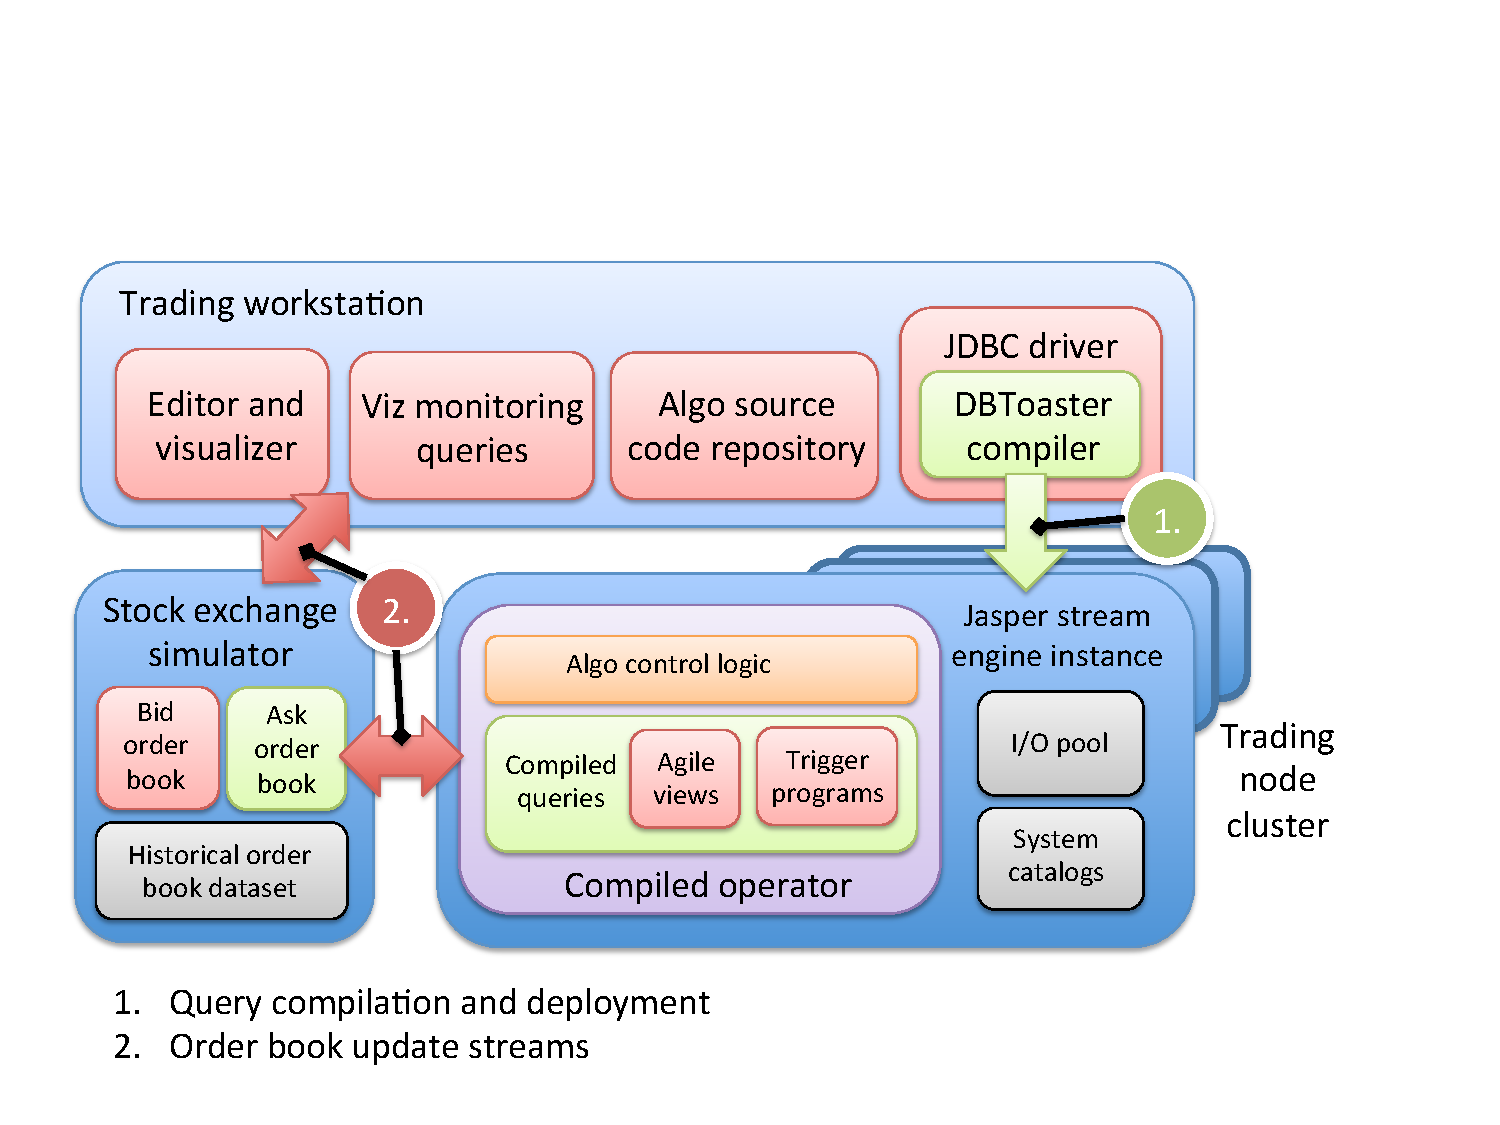
\includegraphics[scale=0.38]{figures/algo-arch}
\end{center}
\label{fig:algarch}
\vspace{-5mm}
\caption{Algorithmic trading platform design.}
\end{figure}


\tinysection{Algorithmic trading workflow}
Figure~\ref{fig:algarch} is an architecture diagram of our algorithmic trading
platform built on top of the \compiler\ platform. To summarize the workflow
described for the three components above, algo developers and traders use the
trading workstation to submit new algos to the trading platform runtime and
monitor their behavior. The trading platform runtime is the \compiler runtime as
described in Section~\ref{sec:dbtoaster} executing algos compiled into
\targetlang\ operators. In addition to \compiler\ trigger programs maintaining
agile views and query results, these operators may include messaging and control
logic to perform tasks such as smart order routing across multiple exchanges.
The trading platform maintains input streams coming from each exchange in the
system to provide a read-only copy of each exchange's order books. The trading
platform provides output streams to each exchange through which algos can send
order requests and modifications. Finally the stock exchange simulator accepts
new and updates to orders on its input streams, applies a matching process to
enact trading, and reflects the status of the order books to all subscribers. 


\section{Demo Scenario}

\todo{Demo screenshots}

\tinysection{Audience Participation}


\bibliographystyle{abbrv}
\bibliography{ref}


\end{document}
